\thispagestyle{thachthuctoanhocnone}
\pagestyle{thachthuctoanhoc}
\everymath{\color{thachthuctoanhoc}}
\graphicspath{{../thachthuctoanhoc/pic/}}
\begingroup
\AddToShipoutPicture*{\put(0,616){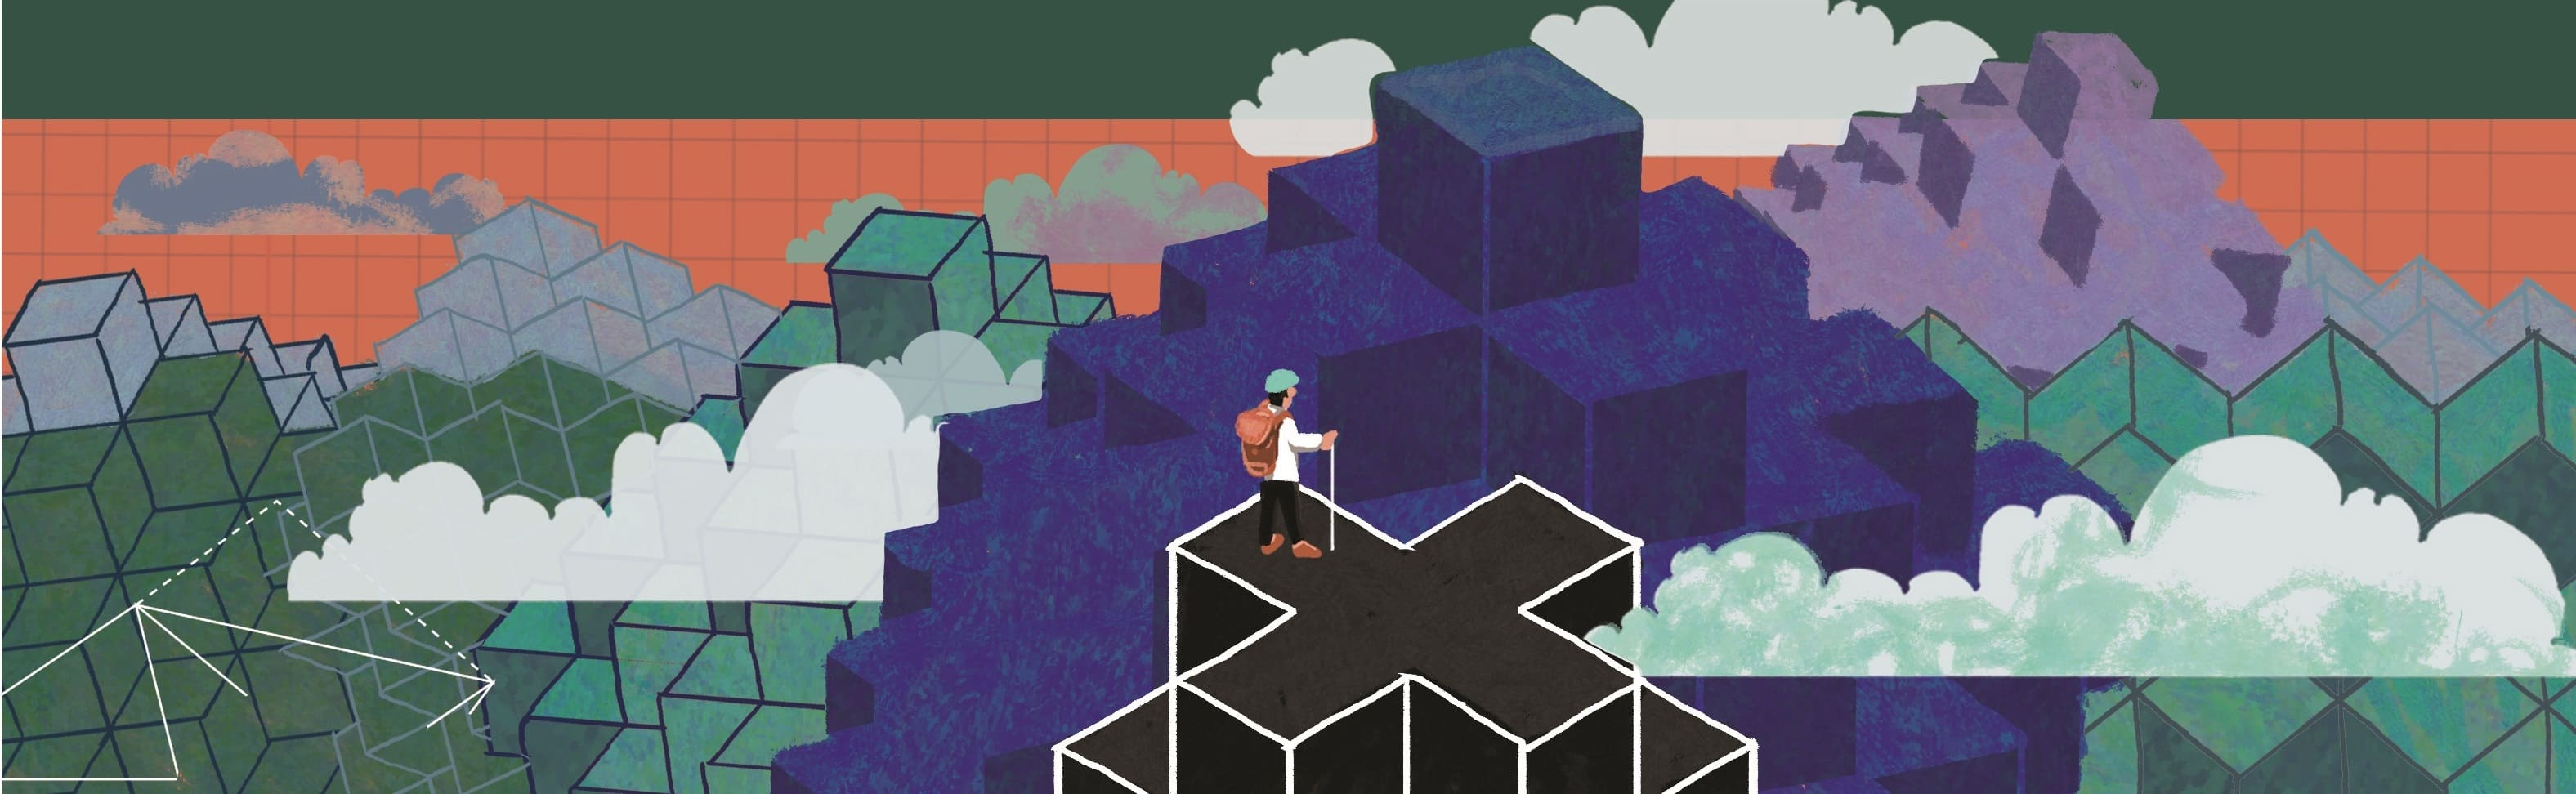
\includegraphics[width=19.3cm]{../thachthuctoanhoc/bannerthachthuc}}}
\centering
\vspace*{4cm}
\endgroup
\vspace*{-8pt}
\begin{tBox}
	\begin{itemize}[leftmargin = 13pt, itemsep = 1.0pt] 
		%		\item Mỗi bài toán đề xuất (kèm theo lời giải) cần được nêu rõ là bài sáng tác hay bài sưu tầm.
		\item Mỗi bài toán đề xuất (kèm theo lời giải) cần được nêu rõ là bài sáng tác hay bài sưu tầm (nếu là bài sưu tầm, cần ghi rõ nguồn).
		\item Bài giải cho mỗi bài toán cần được trình bày trong một file riêng hoặc
		một tờ giấy riêng.
		\item  Người đề xuất bài toán hoặc gửi bài giải cho các bài toán trong mục ``Thách thức kỳ này" cần ghi rõ họ, đệm, tên và nơi làm việc/học tập, số điện thoại liên hệ. Nếu là học sinh (hoặc sinh viên) cần ghi rõ là học sinh lớp mấy (hoặc sinh viên năm thứ mấy).
		\item Các bài toán trong mục Thách thức kỳ này hướng tới các độc giả là học sinh phổ thông; được phân chia thành các mức độ $B$, $A$, và được sắp xếp theo độ khó tăng dần, theo đánh giá chủ quan của Ban biên tập. Các bài toán mức độ $B$ không đòi hỏi các kiến thức vượt quá chương trình môn Toán cấp THCS; các bài toán mức độ $A$ không đòi hỏi các kiến thức vượt quá chương trình môn Toán cấp THPT.
		\item Cách thức gửi bài toán đề xuất hoặc lời giải: gửi file thu được bằng cách scan, ảnh chụp (rõ nét) của bản viết tay, hoặc được soạn thảo bằng các phần mềm Latex, Word tới \url{bbt@pi.edu.vn} hoặc gửi qua đường bưu điện tới Tòa soạn (xem địa chỉ tại bìa $2$).
		\item Hạn gửi lời giải cho các bài toán P$611$--P$620$: trước ngày $15/8/2022$.
	\end{itemize}
\end{tBox}
\begin{center}
	\vspace*{-5pt}
	\textbf{\color{thachthuctoanhoc}THÁCH THỨC KỲ NÀY}
	\vspace*{-5pt}
\end{center}
\begin{multicols}{2}
	\setlength{\abovedisplayskip}{4pt}
	\setlength{\belowdisplayskip}{4pt}
	{\color{thachthuctoanhoc}{\usefont{T5}{qag}{b}{n} P611.}}
	(Mức $B$) Cho $A,B,C$ là các chữ số khác $0$ sao cho $\overline{CCA}+\overline{B2B}=\overline{A88}$. Hãy tìm số $\overline{ABC}$. 
	\vskip 0.05cm
	\hfill	\textit{Tường Thanh, Nghệ An (st)}
	\vskip 0.05cm
	{\color{thachthuctoanhoc}{\usefont{T5}{qag}{b}{n} P612.}}
	(Mức $B$) Chứng minh biểu thức sau nhận giá trị nguyên với mọi giá trị nguyên dương của $n$
	\begin{align*}
		A\!=\!\dfrac{\left(2^4\!+\!\dfrac14\right)\!\left(4^4\!+\!\dfrac14\right)\!\cdots\! \left((2n)^4\!+\!\dfrac14\right)}{\left(1^4\!+\!\dfrac14\right)\left(3^4\!+\!\dfrac14\right)\!\cdots\! \left((2n\!-\!1)^4\!+\!\dfrac14\right)}.
	\end{align*}
	\vskip 0.05cm
	\hfill	\textit{Phùng Chí Tự, Hà Nội (st)}
	\vskip 0.05cm
	{\color{thachthuctoanhoc}{\usefont{T5}{qag}{b}{n} P613.}}
	(Mức $B$) Cho $n$ là một số nguyên dương. Chứng minh rằng, trong ba số $n$,  $\dfrac{n-5}2$, và $\dfrac{15n-9}7$, có ít nhất hai số không phải là số chính phương.
	\begin{flushright}
		\textit{Trương Quang An, Quảng Ngãi}
	\end{flushright}
	{\color{thachthuctoanhoc}{\usefont{T5}{qag}{b}{n} P614.}}
	(Mức $B$) Cho $a,b$ là các số nguyên dương thoả mãn
	\begin{align*}
		\left\{ \sqrt{a+\sqrt{a}}\right\}=\{\sqrt b\}.
	\end{align*}
	Chứng minh rằng, $4b+1$ là một số chính phương.
	\vskip 0.05cm
	(Với $x$ là một số thực, $\{x\}=x-[x]$, trong đó $[x]$ là số nguyên lớn nhất không vượt quá $x$. Đại lượng $\{x\}$ được gọi là {\it phần lẻ} của số thực $x$)
	\begin{flushright}
		\textit{Lưu Bá Thắng, Hà Nội}
	\end{flushright}
	{\color{thachthuctoanhoc}{\usefont{T5}{qag}{b}{n} P615.}}
	(Mức $B$) Cho tam giác $ABC$ vuông tại $A$. Một điểm $D$ di chuyển trên tia $CA$. Gọi $E$ là hình chiếu vuông góc của điểm $C$ trên đường thẳng $BD$; $F$ là giao điểm của $AE$ và $BC$. Chứng minh rằng, đường thẳng $DF$ luôn đi qua một điểm cố định.
	\begin{figure}[H]
		\vspace*{-5pt}
		\centering
		\captionsetup{labelformat= empty, justification=centering}
%		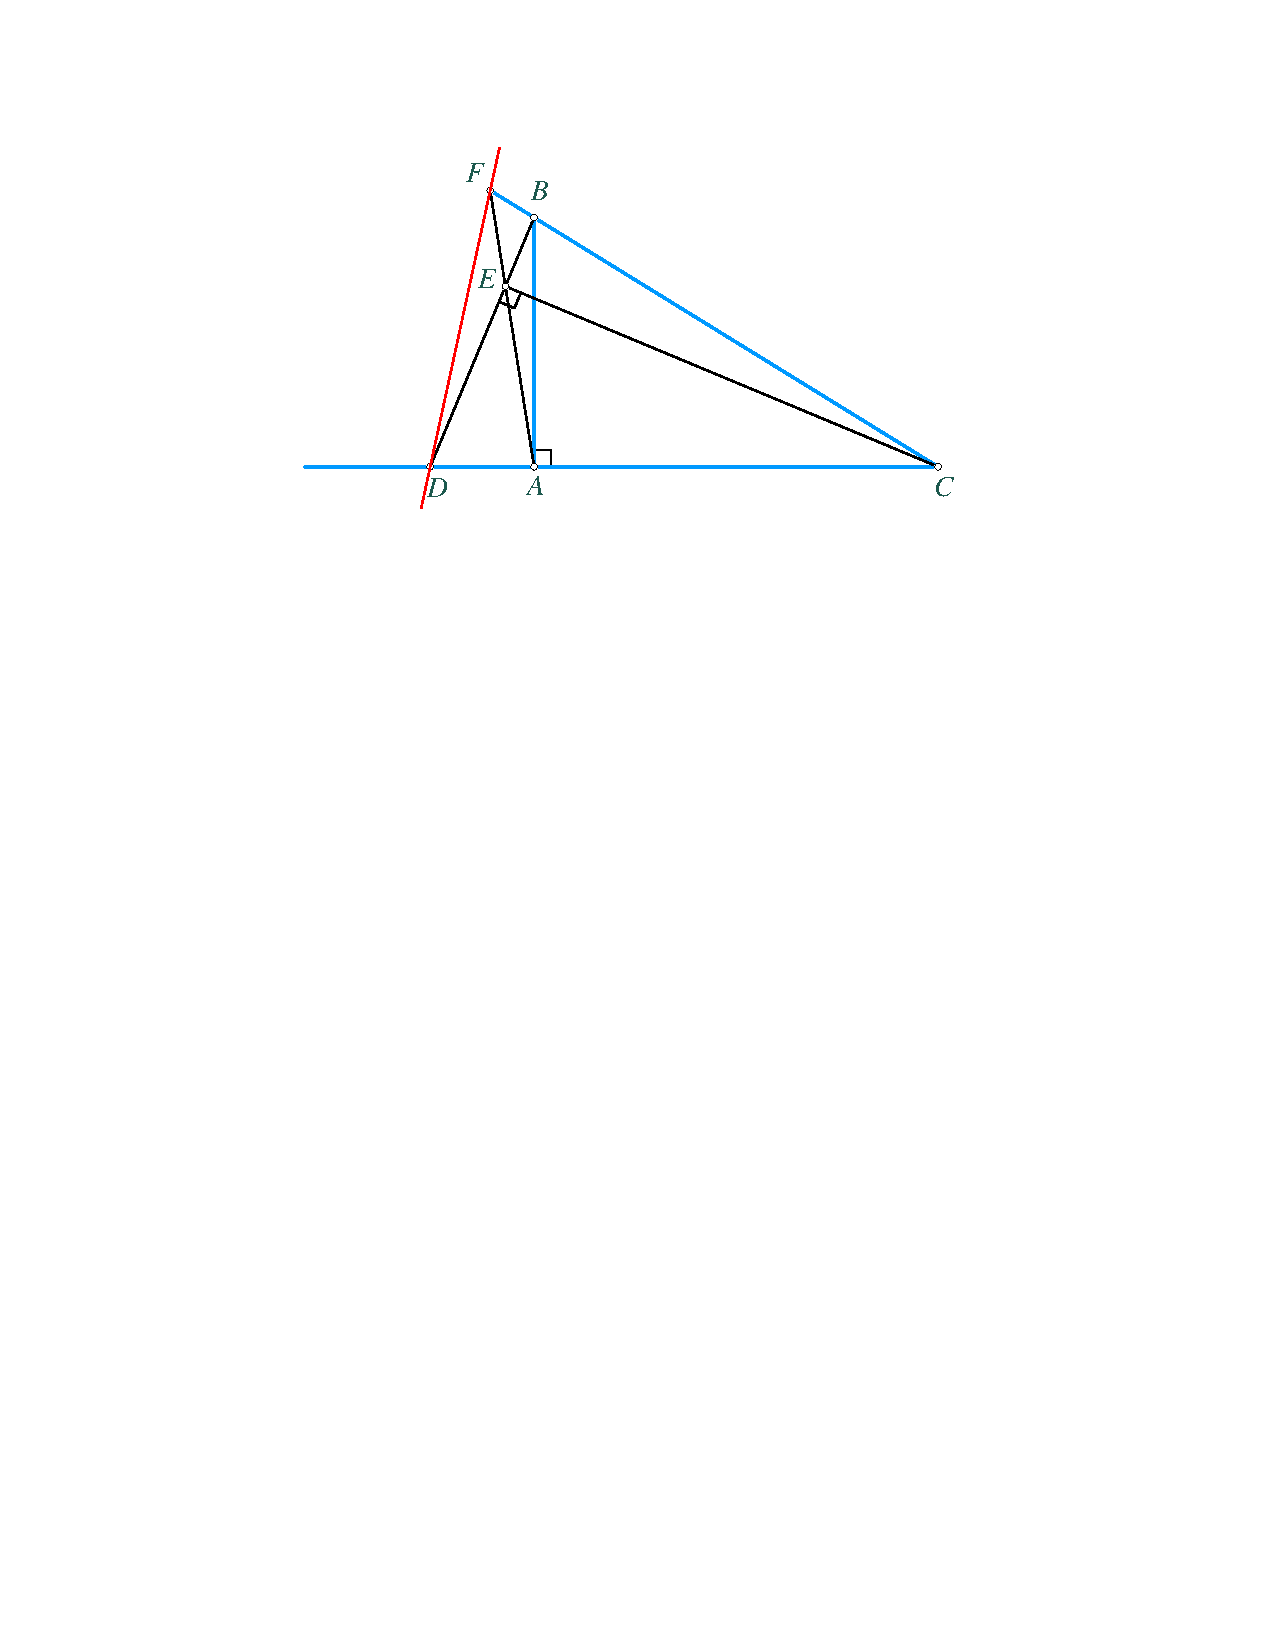
\includegraphics[width= 1\linewidth]{P615}
		\vspace*{-15pt}
	\end{figure}
	\hfill	\textit{Trần Thanh Hưng, Phú Yên}
	\vskip 0.05cm
	{\color{thachthuctoanhoc}{\usefont{T5}{qag}{b}{n} P616.}}
	(Mức $B$) Xét các số dương $a,b,c$ thoả mãn $a+b+c=4$. Tìm giá trị nhỏ nhất của biểu thức 
	\begin{align*}
		P=\left|\dfrac 1a-1\right|+\left|\dfrac 1b-1\right|+\left|\dfrac 1c-1\right|.
	\end{align*}
	\begin{flushright}
		\textit{Nguyễn Tuấn Ngọc, Tiền Giang}
	\end{flushright}
	{\color{thachthuctoanhoc}{\usefont{T5}{qag}{b}{n} P617.}}
	(Mức $A$) Giải phương trình
	\begin{align*}
		\sqrt{(x^3-4)^3}=\sqrt[3]{(x^2+4)^2}+4.
	\end{align*} 
	\begin{flushright}
		\textit{Trần Văn Lâm, Thái Nguyên (st)}
	\end{flushright}
	{\color{thachthuctoanhoc}{\usefont{T5}{qag}{b}{n} P618.}}
	(Mức $A$) Cho $a,b,c$ là các số nguyên lớn hơn $1$. Giả sử $x,y,z$ là các số thực thoả mãn $a^x=bc$, $b^y=ca$ và $c^z=ab$. Tính giá trị của biểu thức $T=x+y+z-xyz$. 
	\vskip 0.05cm
		\hfill \textit{Bằng Linh, Phú Thọ (st)}
	\vskip 0.05cm
	\columnbreak
	{\color{thachthuctoanhoc}{\usefont{T5}{qag}{b}{n} P619.}}
	(Mức $A$) Cho tam giác $ABC$ nội tiếp đường tròn $(O)$, có trực tâm $H$. Gọi $M$ là điểm chính giữa cung $BAC$ của $(O)$. Qua $O$ kẻ đường thẳng  song song với $AM$, cắt $HM$ tại $P$. Gọi $X,Y,Z$ tương ứng là hình chiếu vuông góc của $P$ trên $BC,CA,AB$. Chứng minh rằng đường tròn ngoại tiếp tam giác $XYZ$ đi qua trung điểm của $HM.$
	\begin{figure}[H]
		\vspace*{-10pt}
		\centering
		\captionsetup{labelformat= empty, justification=centering}
%		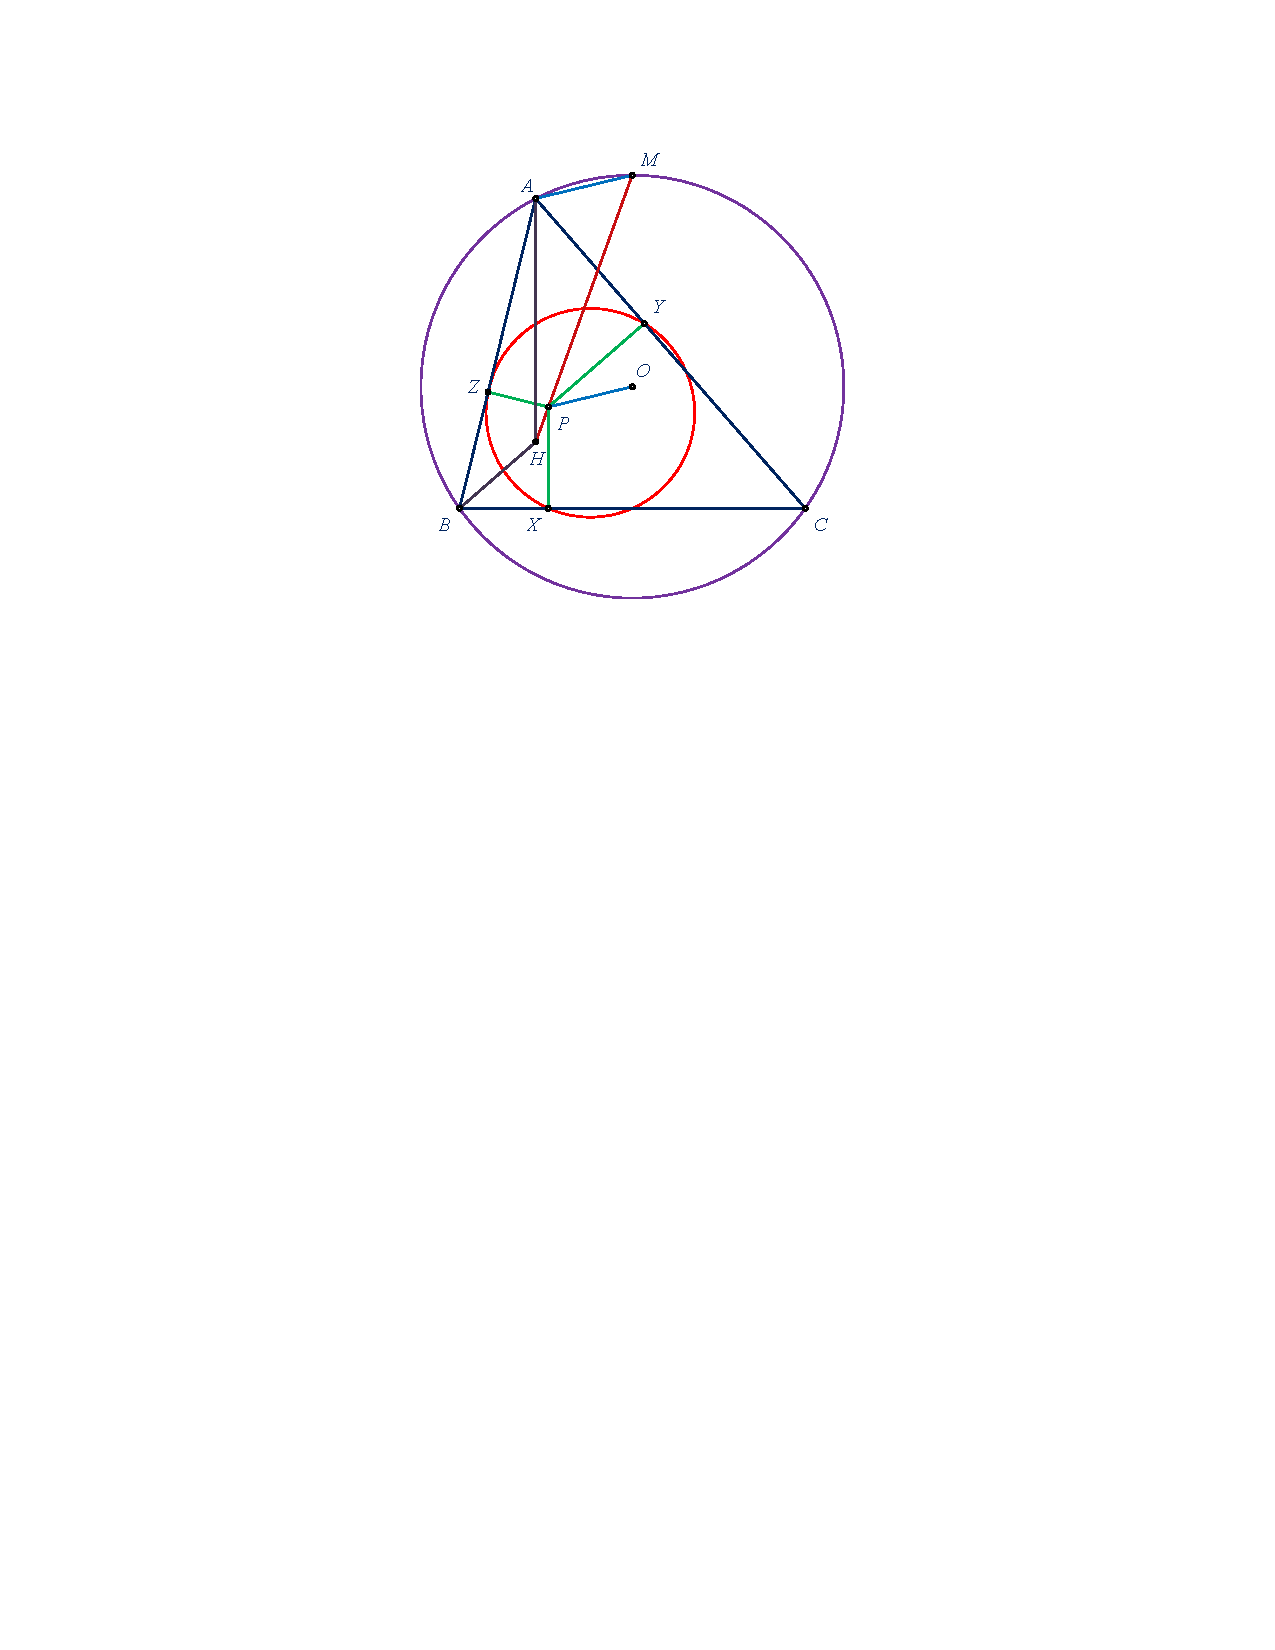
\includegraphics[width= 1\linewidth]{P619}
		\vspace*{-15pt}
	\end{figure}
	\begin{flushright}
		\textit{Nguyễn Văn Linh, Hà Nội}
	\end{flushright}
	{\color{thachthuctoanhoc}{\usefont{T5}{qag}{b}{n} P620.}}
	(Mức $A$) Chứng minh rằng với mọi số nguyên tố $p\ge5$, tồn tại số nguyên $t$ sao cho: với mọi số nguyên $k$ thì $k^2-2t^2-1$ không chia hết cho $p$.   
	\begin{flushright}
		\textit{Nguyễn Quang Minh, Singapore}
	\end{flushright}
\end{multicols}
\begin{center}
	{\large{\textbf{\color{thachthuctoanhoc}\color{thachthuctoanhoc}GIẢI BÀI KỲ TRƯỚC}}}
\end{center}
\begin{multicols}{2}
	\setlength{\abovedisplayskip}{4pt}
	\setlength{\belowdisplayskip}{4pt}
	{\color{thachthuctoanhoc}{\usefont{T5}{qag}{b}{n} P591.}}
	(Mức $B$) Xét bốn số thực phân biệt có tính chất: Mỗi số $189$, $264$, $287$, $320$ đều là tổng của hai trong bốn số ấy. Hỏi, tổng của bốn số đó có thể lớn nhất là bao nhiêu?
	\vskip 0.05cm
	\textbf{Lời giải} \textit{(phỏng theo ý giải của bạn Trần Minh Hoàng, lớp $9$E, trường THCS Nguyễn Trãi, Huyện Nghi Xuân, Tỉnh Hà Tĩnh})\textbf{.}
	\vskip 0.05cm
	Gọi $a$, $b$, $c$, $d$ là bốn số thực có tính chất đã nêu trong đề bài.
	\vskip 0.05cm
	Khi đó, $189$, $264$, $287$, $320$ là bốn trong sáu số: $a + b$, $c + d$, $a + c$, $b + d$, $a + d$, $b + c$. Do đó, bốn số vừa nêu thuộc ba nhóm số $\{a \!+\! b; c \!+\! d\}$, $\{a \!+\! c; b \!+\! d\}$ và $\{a \!+\! d; b \!+\! c\}$. Suy ra, phải có hai trong bốn số ấy thuộc cùng một nhóm. Do hai số đó là hai số phân biệt nên tổng của chúng chính là tổng của hai số trong nhóm. Từ đây, vì tổng của hai số cùng nhóm nào cũng bằng $a + b + c + d$, nên suy ra trong bốn số $189$, $264$, $287$, $320$ phải có hai số có tổng bằng $a + b + c + d$. Vì thế, ta có:
	\begin{align*}
		a + b + c + d \le 287 + 320 = 607.
	\end{align*}
	Hơn nữa, nhận thấy, bốn số $83$, $106$, $181$, $237$ có tính chất đã nêu trong đề bài (vì $189 = 83 + 106$, $264 = 83 + 181$,\linebreak $287 = 106 + 181$, $320 = 83 + 237$) và tổng của chúng bằng
	\begin{align*}
		83 + 106 + 181 + 237 = 607.
	\end{align*}
	Vì vậy, tổng của bốn số có tính chất đã nêu trong đề bài có thể lớn nhất bằng $607$.
	\vskip 0.05cm
	\textbf{Bình luận và Nhận xét}
	\vskip 0.05cm
	Ngoài lời giải của bạn \textit{Trần Minh Hoàng}, Tạp chí đã nhận được hai lời giải nữa; trong đó, có một lời giải sai, và một lời giải không được chấp nhận là lời giải hoàn chỉnh, vì mắc lỗi logic (cụ thể, người giải bài đã khẳng định, giá trị lớn nhất của tổng $a + b + c + d$ bằng $607$ ngay sau khi mới chỉ chứng minh được tổng đó không vượt quá $607$).
	\begin{flushright}
		\textbf{Lê Huy}
	\end{flushright}
	{\color{thachthuctoanhoc}{\usefont{T5}{qag}{b}{n} P592.}}
	(Mức $B$) Tìm chữ số hàng đơn vị của số
	\begin{align*}
		A = &\left( {1 + {2^2} + {3^3} +  \cdots  + {{2022}^{2022}}} \right)\\
		&\times\!\left( {{5^5} + {{15}^{15}} + {{25}^{25}} +  \cdots  + {{2025}^{2025}}} \right)\!.
	\end{align*}
	\textbf{Lời giải} (\textit{dựa theo lời giải của bạn Hà Mạnh Hùng, lớp $7$A, trường THPT chuyên Hà Nội -- Amsterdam, Tp. Hà Nội})\textbf{.}
	\vskip 0.05cm
	Đặt  $B = 1 + {2^2} + {3^3} +  \cdots  + {2022^{2022}}$ và $C = {5^5} + {15^{15}} + {25^{25}} +  \cdots  + {2025^{2025}}$.
	\vskip 0.1cm 
	Ta có:
	\begin{align*}
		B = &\left( {1 + {2^2}} \right) + \left( {{3^3} + {4^4}} \right) +  \cdots\\
		  &+ \left( {{{2021}^{2021}} + {{2022}^{2022}}} \right).
	\end{align*}
	Dễ thấy, tổng của hai số trong mỗi ``ngoặc đơn" là một số lẻ, và có tất cả $2022 : 2 = 1011$ ``ngoặc đơn". Do đó, $B$ là tổng của một số lẻ các số lẻ. Vì thế, $B$ là một số lẻ.   \hfill ($1$)
	\vskip 0.05cm
	Tiếp theo, nhận thấy, mỗi số hạng của tổng $C$ là một số lẻ chia hết cho $5$, và tổng đó có $(2025 - 5) : 10 + 1 = 203$ số hạng. Do đó, $C$ là tổng của một số lẻ các số lẻ chia hết cho $5$. Vì thế, $C$ là một số lẻ, chia hết cho $5$. \hfill ($2$)
	\vskip 0.05cm
	Từ ($1$) và ($2$) suy ra, $A = B \cdot C$  là một số lẻ, chia hết cho $5$. Vì thế, chữ số tận cùng, hay chữ số hàng đơn vị, của $A$ là $5$.
	\vskip 0.05cm
	\textbf{Bình luận và Nhận xét}
	\vskip 0.05cm
	Tất cả các lời giải Tạp chí nhận được từ bạn đọc đều có ý giải đúng. Tuy nhiên, một số lời giải trong số đó không được chấp nhận là lời giải hoàn chỉnh do người giải bài đã tính sai số số hạng của tổng $C$ (trong lời giải trên), hoặc lời giải được trình bày quá vắn tắt, thiếu các lí giải cần thiết.
	\begin{flushright}
		\textbf{Lưu Thị Thanh Hà}
	\end{flushright}
	{\color{thachthuctoanhoc}{\usefont{T5}{qag}{b}{n} P593.}}
	(Mức $B$) Cho $n$ là một số nguyên dương. Chứng minh rằng, nếu $4n + 1$ và $20n + 1$ là các số chính phương thì $20n + 21$ là một hợp số.
	\vskip 0.05cm
	\textbf{Lời giải} (\textit{dựa theo lời giải của bạn Trần Minh Hoàng, lớp $9$E, trường THCS Nguyễn Trãi, Huyện Nghi Xuân, Tỉnh Hà Tĩnh})\textbf{.}
	\vskip 0.05cm
	Ta biết rằng, khi chia một số chính phương cho $3$ sẽ được số dư là $0$ hoặc $1$. Vì thế, từ giả thiết $4n + 1$ và $20n + 1$ là các số chính phương, suy ra, hoặc $4n + 1$ và $20n + 1$ cùng chia hết cho $3$ (tức, chia $3$ dư $0$), hoặc trong hai số $4n + 1$ và $20n + 1$ có ít nhất một số chia $3$ dư $1$.
	\vskip 0.1cm
	Nếu $4n + 1$ và $20n + 1$ cùng chia hết cho $3$ thì
	\begin{align*}
		(20n + 1) - (4n + 1) = 16n
	\end{align*}
	chia hết cho $3$. Suy ra, $n$ chia hết cho $3$ (do $16$ và $3$ nguyên tố cùng nhau). Vì thế, $4n$ và $20n$ chia hết cho $3$; suy ra, $1$ chia hết cho $3$, là điều vô lí. Vì vậy, phải có: trong hai số $4n + 1$ và $20n + 1$ có ít nhất một số chia $3$ dư $1$. Khi đó, trong hai số $4n$ và $20n$ có ít nhất một số chia hết cho $3$. Từ đây, vì $4$ và $3$ nguyên tố cùng nhau, $20$ và $3$ nguyên tố cùng nhau, suy ra, $n$ chia hết cho $3$. Vì thế, $20n + 21$ chia hết cho $3$. Mà $20n + 21 > 3$, nên $20n + 21$ là hợp~số.
	\vskip 0.05cm
	Ta có điều phải chứng minh theo yêu cầu đề bài.
	\vskip 0.05cm
	\textbf{Bình luận và Nhận xét}
	\vskip 0.05cm
	Rất tiếc, trong số các lời giải Tạp chí đã nhận được từ bạn đọc, có một lời giải sai, do người giải bài đã mắc \textbf{\textit{lỗi}} sau: ``Với $a$, $b$, $c$ là các số nguyên dương, từ  $a = b \cdot c$ và $b > 1$, suy ra, $a$ là hợp số.". (\textit{Khẳng định vừa nêu hiển nhiên sai, nếu $c = 1$ và $b$ là số nguyên tố.}). Ngoài lời giải sai vừa nêu, tất cả các lời giải còn lại đều là lời giải đúng và hoàn chỉnh.
	\begin{flushright}
		\textbf{Lưu Thị Thanh Hà}
	\end{flushright}
	{\color{thachthuctoanhoc}{\usefont{T5}{qag}{b}{n} P594.}}
	(Mức $B$) Giải phương trình:
	\begin{align*}
		&\sqrt {1 + 2x}  + \sqrt {1 - 2x}  \\
		= \,&\left( {1 + 3x} \right)\sqrt {1 - 3x}  + \left( {1 - 3x} \right)\sqrt {1 + 3x} .
	\end{align*}
	\textbf{Lời giải} (\textit{dựa theo cách giải của bạn Nguyễn Đức Khải, lớp $10$T$2$, trường THPT chuyên Lê Hồng Phong, Tỉnh Nam Định}).
	\vskip 0.05cm
	Điều kiện xác định của phương trình:
	\begin{align*}
		-\dfrac{1}{3} \le x \le \dfrac{1}{3}.
	\end{align*}
	Với điều kiện đó, phương trình đã cho tương đương với phương trình
	\begin{align*}
		&\sqrt {1 + 2x}  + \sqrt {1 - 2x}  \\
		= \,&\sqrt {1 - 9{x^2}} \left( {\sqrt {1 + 3x}  + \sqrt {1 - 3x} } \right).
	\end{align*}
	Vì thế, giả sử $x_0$  là nghiệm của phương trình đã cho, ta có $ - \dfrac{1}{3} \le {x_0} \le \dfrac{1}{3}$  và
	\begin{align*}
		&\sqrt {1 + 2{x_0}}  + \sqrt {1 - 2{x_0}}  \\
		= \,&\sqrt {1 - 9x_0^2} \left( {\sqrt {1 + 3{x_0}}  + \sqrt {1 - 3{x_0}} } \right). \tag{$1$}
	\end{align*}
	Kí hiệu $VP$ là vế phải của ($1$).\\
	Do $0 \le \sqrt {1 - 9x_0^2}  \le 1$  nên
	\begin{align*}
		VP \le \sqrt {1 + 3{x_0}}  + \sqrt {1 - 3{x_0}} .
	\end{align*}
	Do đó, từ ($1$) suy ra
	\begin{align*}
		\sqrt {\!1 \!+\! 2{x_0}}  \!+\!\! \sqrt {\!1 \!-\! 2{x_0}}  \!\le\!\! \sqrt {\!1 \!+\! 3{x_0}}  \!+\!\! \sqrt {\!1 \!-\! 3{x_0}} .
	\end{align*}
	Ta có:
	\begin{align*}
		(2) &\Leftrightarrow 2 + 2\sqrt {1 - 4x_0^2}  \le 2 + 2\sqrt {1 - 9x_0^2} \\
		&\Leftrightarrow \sqrt {1 - 4x_0^2}  \le \sqrt {1 - 9x_0^2} \\
		&\Leftrightarrow 1 - 4x_0^2 \le 1 - 9x_0^2 \Leftrightarrow x_0^2 \le 0.
	\end{align*}  
	Vì thế,  $x_0 = 0$.
	\vskip 0.05cm
	Ngược lại, bằng cách thử trực tiếp, ta thấy, $x = 0$ nghiệm đúng phương trình đã cho.
	\vskip 0.05cm
	Vậy, phương trình đã cho có duy nhất nghiệm $x = 0$.
	\vskip 0.05cm
	\textbf{Bình luận và Nhận xét}
	\vskip 0.05cm
	$\pmb{1.}$ Hầu hết các lời giải Tạp chí đã nhận được từ bạn đọc đều là lời giải theo cách sử dụng phép bình phương hai vế của phương trình để thực hiện các biến đổi tương đương. Lời giải theo cách này khá dài dòng và cồng kềnh.
	\vskip 0.05cm
	$\pmb{2.}$ Tất cả các lời giải Tạp chí nhận được từ bạn đọc đều là lời giải đúng và hoàn chỉnh.
	\begin{flushright}
		\textbf{Lê Huy}
	\end{flushright}
	{\color{thachthuctoanhoc}{\usefont{T5}{qag}{b}{n} P595.}}
	(Mức $B$) Cho tam giác nhọn, không cân $ABC$, nội tiếp đường tròn $(O)$, có các đường cao $AD$, $BE$, $CF$. Gọi $G$ là giao điểm của các đường thẳng $BC$, $EF$. Đường tròn ngoại tiếp tam giác $ADG$ cắt $(O)$ tại điểm thứ hai $I$ (khác $A$). Các đường thẳng $AI$ và $EF$ cắt nhau tại $K$. Chứng minh rằng, đường thẳng nối $K$ và trực tâm của tam giác $ABC$ đi qua trung điểm của $BC$.
	\vskip 0.05cm
	\textbf{Lời giải} ()\textbf{.}
	\vskip 0.05cm
	
	\textbf{Bình luận và Nhận xét}
	
	\begin{flushright}
		\textbf{Hạ Vũ Anh}
	\end{flushright}
	{\color{thachthuctoanhoc}{\usefont{T5}{qag}{b}{n} P596.}}
	(Mức $B$) Cho các số thực không âm $a, b, c$, thỏa mãn $a^2 + b^2 + c^2 =2$.  Chứng minh rằng
	\begin{align*}
		8\left( {2 \!-\! a \!-\! b} \right)\left( {2 \!-\! b \!-\! c} \right)\left( {2 \!-\! c \!-\! a} \right) \ge {\left( {abc} \right)^2}.
	\end{align*}
	Dấu đẳng thức xảy ra khi nào?
	\vskip 0.05cm
	\textbf{Lời giải} (\textit{dựa theo cách giải của đa số lời giải Tạp chí đã nhận được từ bạn đọc})\textbf{.}
	\vskip 0.05cm
	Từ giả thiết của bài ra, ta có:
	\begin{align*}
		&2\left( {2 - a - b} \right) \\
		= \,&4 - 2a - 2b \\
		= \,&{a^2} + {b^2} + {c^2} - 2a - 2b + 2 \\
		= \,&{\left( {a - 1} \right)^2} + {\left( {b - 1} \right)^2} + {c^2} \ge {c^2}. \tag{$1$}
	\end{align*}
	Bằng cách hoàn toàn tương tự, ta cũng chứng minh được:
	\begin{align*}
		&2\left( {2 - b - c} \right) \ge {a^2}.\tag{$2$}\\
		&2\left( {2 - c - a} \right) \ge {b^2}.\tag{$3$}
	\end{align*}
	Vì các vế của các bất đẳng thức cùng chiều ($1$), ($2$), ($3$) đều là các số không âm (do  $a^2$, $b^2$, $c^2 \ge 0$), nên nhân các bất đẳng thức đó, vế theo vế, ta nhận được bất đẳng thức cần chứng minh theo yêu cầu đề bài.
	\vskip 0.05cm
	Dễ thấy, dấu đẳng thức xảy ra khi và chỉ khi trong ba số $a, b, c$ có hai số bằng $1$ và số còn lại bằng $0$.
	\vskip 0.05cm
	\textbf{Bình luận và Nhận xét}
	\vskip 0.05cm
	Rất tiếc, trong số các lời giải Tạp chí đã nhận được từ bạn đọc, có một lời giải không được chấp nhận là lời giải hoàn chỉnh, do người giải bài chưa nêu câu trả lời cho câu hỏi ``Dấu đẳng thức xảy ra khi nào?" của đề bài. Tất cả các lời giải còn lại đều là lời giải hoàn chỉnh.
	\begin{flushright}
		\textbf{Lê Huy}
	\end{flushright}
	{\color{thachthuctoanhoc}{\usefont{T5}{qag}{b}{n} P597.}}
	(Mức $A$) Một nhà địa chất đang ở vị trí $A$ trong sa mạc, cách con đường thẳng $10km$ ($AN = 10km$). Trên con đường đó, xe của nhà địa chất có thể chạy với vận tốc tối đa $50km/h$, nhưng trên sa mạc nó chỉ chạy được với vận tốc tối đa $30km/h$.
	\begin{figure}[H]
		\centering
		\vspace*{-10pt}
		\captionsetup{labelformat= empty, justification=centering}
		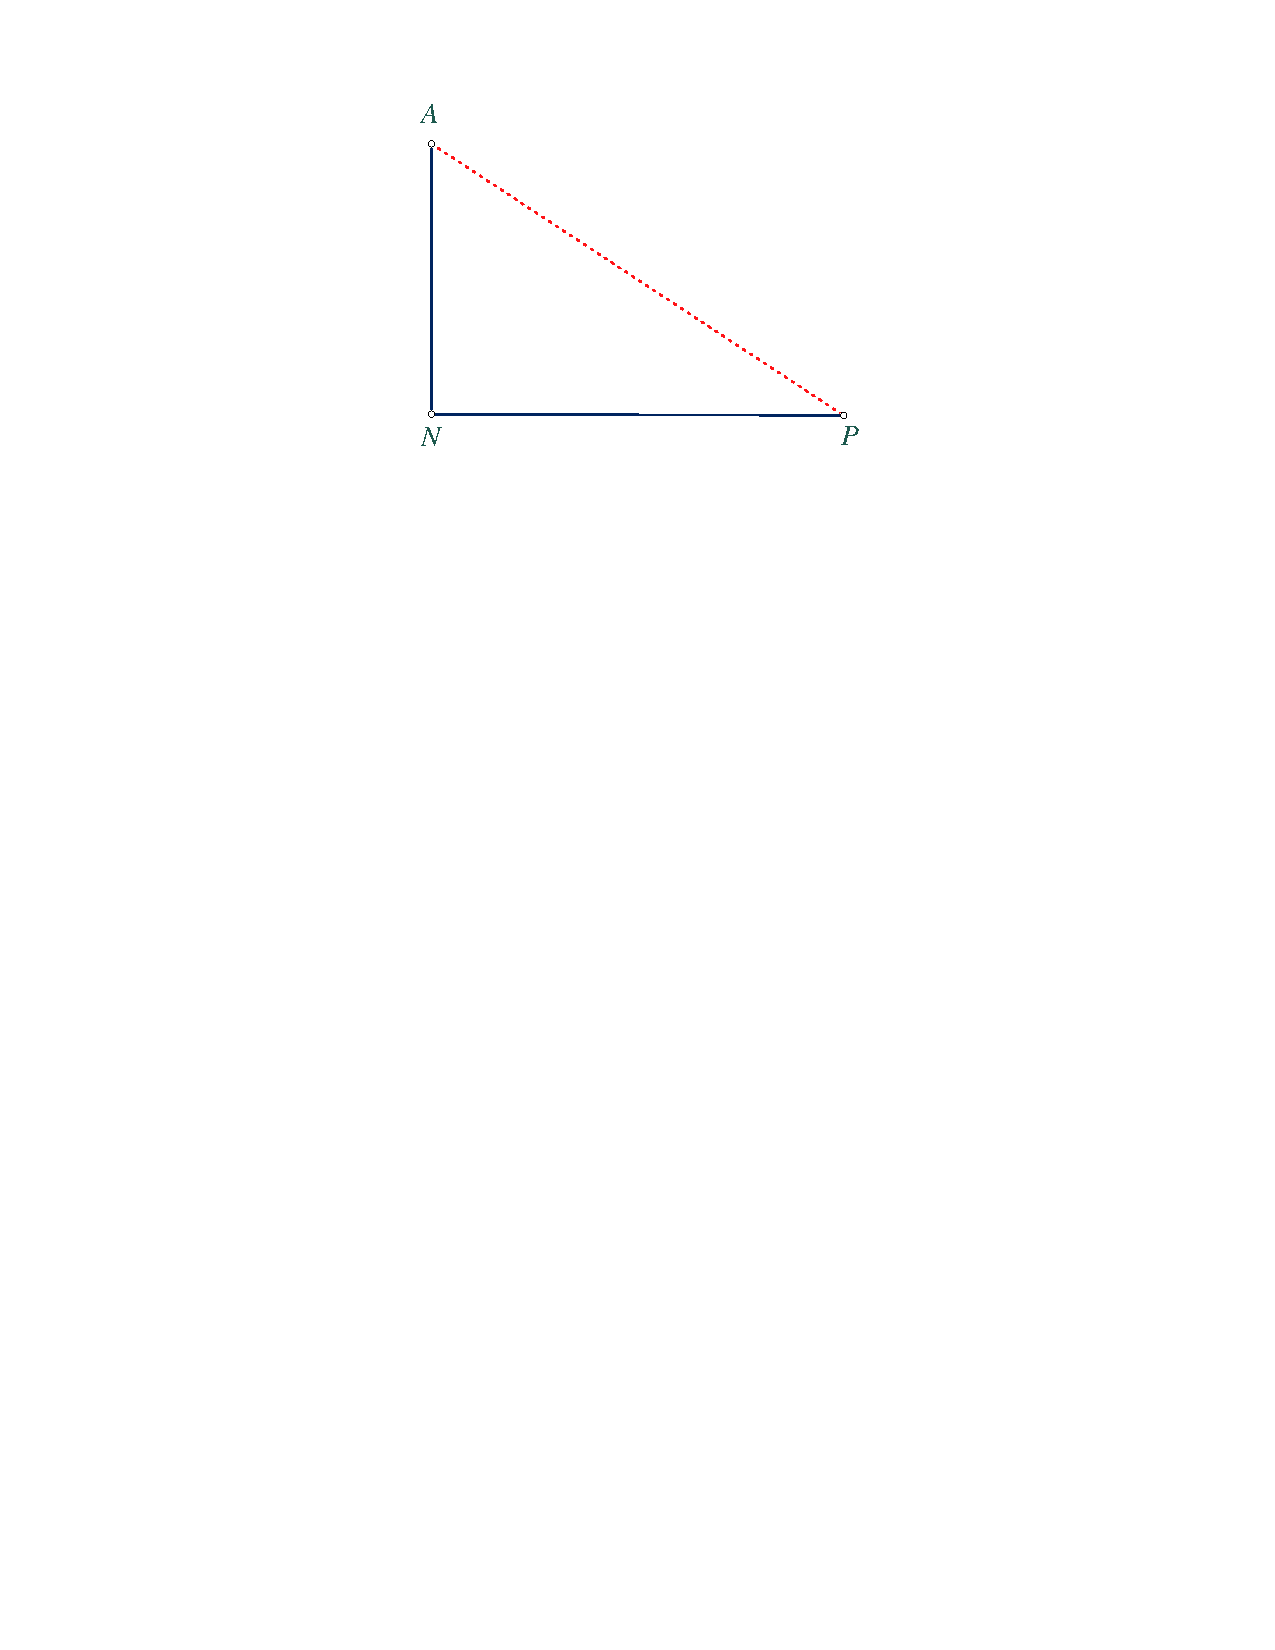
\includegraphics[width=0.75\linewidth]{P597}
		\vspace*{-5pt}
	\end{figure}
	Nhà địa chất đang rất khát nước, và ông biết rằng, có một trạm xăng $P$ ở vị trí xuôi theo đường $25km$ ($NP = 25km$), và ở đó có bán nước giải khát.
	\vskip 0.05cm
	$a)$ Nhà địa chất cần ít nhất bao nhiêu phút, để đi từ $A$ đến $P$ theo đường sa mạc?
	\vskip 0.05cm
	$b)$ Nếu nhà địa chất đi từ $A$ đến $N$, rồi đi theo con đường thẳng để đến $P$ thì có nhanh hơn không?
	\vskip 0.05cm
	$c)$ Hãy tìm một cách đi nhanh hơn cho nhà địa chất. Cách của bạn đã là nhanh nhất chưa?
	\vskip 0.05cm
	\textbf{Lời giải} ()\textbf{.}
	\vskip 0.05cm
	
	\textbf{Bình luận và Nhận xét}
	
	\begin{flushright}
		\textbf{Trần Nam Dũng}
	\end{flushright}
	{\color{thachthuctoanhoc}{\usefont{T5}{qag}{b}{n} P598.}}
	(Mức $A$) Chứng minh rằng, tồn tại số tự nhiên có $2022$ chữ số, được tạo thành từ hai chữ số $4$, $5$, và chia hết cho $2^{2022}$. 
	\vskip 0.05cm
	\textbf{Lời giải} ()\textbf{.}
	
	\textbf{Bình luận và Nhận xét}
	\begin{flushright}
		\textbf{Nguyễn Khắc Minh}
	\end{flushright}
	{\color{thachthuctoanhoc}{\usefont{T5}{qag}{b}{n} P599.}}
	(Mức $A$) Cho các số thực dương $a$, $b$, $c$ có tổng bằng $7$. Chứng minh rằng
	\begin{align*}
		\frac{a}{b} + \frac{b}{c} + \frac{c}{a} + abc \ge ab + bc + ca - 2.
	\end{align*}
	\textbf{Lời giải} ()\textbf{.}
	\vskip 0.05cm
	
	\textbf{Bình luận và Nhận xét}
	\vskip 0.05cm
	
	\begin{flushright}
		\textbf{Võ Quốc Bá Cẩn}
	\end{flushright}
	{\color{thachthuctoanhoc}{\usefont{T5}{qag}{b}{n} P600.}}
	(Mức $A$) Cho $A$ là một tập con có $100$ phần tử của tập hợp gồm $178$ số nguyên dương đầu tiên. Chứng minh rằng, với mỗi số $n$ thuộc tập hợp gồm $24$ số nguyên dương đầu tiên, đều tồn tại hai số thuộc $A$, có hiệu bằng $n$.
	\vskip 0.05cm
	\textbf{Lời giải} ()\textbf{.}
	\vskip 0.05cm
	
	\textbf{Bình luận và Nhận xét}
	\vskip 0.05cm
	\begin{flushright}
		\textbf{Nguyễn Khắc Minh}
	\end{flushright}
\end{multicols}

